\documentclass{beamer}
\usetheme{metropolis}
\usepackage{latexsym}
\usepackage{amssymb}
\usepackage{amsbsy}
\usepackage{alltt}
\usepackage{tikz}
\usetikzlibrary{shapes}
\usepackage{stmaryrd}
\usepackage{graphicx}

\newcommand{\imp}{\Rightarrow}
\newcommand{\etal}{\textit{et. al}}
\newcommand{\adhoc}{\textit{ad hoc}}
\newcommand{\ie}{\textit{i.e.}}
\newcommand{\etc}{\textit{etc}}
\newcommand{\eg}{\textit{e.g.}}
\newcommand{\kemph}[1]{\colorbox{orange}{#1}}
\newcommand{\highlight}[2][orange]{\mathchoice%
  {\colorbox{#1}{$\displaystyle#2$}}%
  {\colorbox{#1}{$\textstyle#2$}}%
  {\colorbox{#1}{$\scriptstyle#2$}}%
  {\colorbox{#1}{$\scriptscriptstyle#2$}}}%

\newcommand{\konst}[1]{\ensuremath{\mbox{\bf{#1}}}}
\newcommand{\nil}{\konst{[\,]}}
\newcommand{\cons}[2]{{#1}\boldsymbol{:}\boldsymbol{:}{#2}}
\newcommand{\hollamb}{\boldsymbol{\lambda}}
\newcommand{\itelse}[3]{\mbox{$\mbox{\tt if}\ {#1}\ \mbox{\tt then}\ {#2}\
    \mbox{\tt else}\ {#3}$}}
\newcommand{\set}[1]{\{ {#1} \}}
\newcommand{\Lang}[1]{\ensuremath{{\cal L}({#1})}}
\newcommand{\LangTheta}[1]{\ensuremath{{\mathcal L}_{\theta}({#1})}}
\newcommand{\inbox}[1] {\begin{center}
                         \framebox{\parbox{0.984\textwidth}{#1}}
                         \end{center}}

% for backslashes in alltt environments
\newcommand{\bs}{\texttt{\symbol{92}}}

\begin{document}

% Title page

\author{Konrad Slind, David Hardin \\ Collins Aerospace}
\date{Jan. 28, 2021}
\title{SafeDocs--CASE Brainstorming}
\maketitle

\begin{frame}\frametitle{Overview}

\begin{enumerate}
\item Security-Enhancing Architectural Transformations in \konst{CASE}
\item Technical Ideas
\item Applications and Future Directions
\end{enumerate}
\end{frame}


\section {Context: Architectural Transformations in CASE}

\begin{frame}\frametitle{System Architecture Languages}
\begin{itemize}

\item General setting: \textbf{Architectural Design Languages}

\item An ADL supports complete, highly abstract, views of a system,
  including hardware, software, (and possibly humans)

\item An architecture model should provide a high-level setting in which
  the \kemph{whole picture} of a system can be surveyed

\item Thus: a place where existing implementations, new design
  features, high-level requirements, implementations, and
  verifications can be combined.

\item Not just boxes and arrows!

\end{itemize}

\end{frame}

\begin{frame}\frametitle{CASE}
\begin{itemize}

\item In the DARPA \textbf{CASE} project we are developing the idea of
  \kemph{Security-Enhancing} transformations on system architecture
  descriptions.

\item Acronym: \colorbox{orange}{SEAT}

\item The goal is to develop a methodology and case studies where
  \begin{itemize}
  \item [$\blacktriangleright$]
       the structure of an existing (legacy) system is captured in an architectural model;

 \item [$\blacktriangleright$] system security is automatically analyzed and any security
   problems are addressed by applying architectural transformations
 \end{itemize}

\item A key aspect is use of formal specification languages and
  automatic synthesis of security mechanisms.

\end{itemize}

\end{frame}

\begin{frame}[fragile]\frametitle{CASE Website}

Check it out:

\begin{verbatim}
  http://loonwerks.com/projects/case.html
\end{verbatim}

\end{frame}


\begin{frame}\frametitle{Architecture Transformations}

An architecture-to-architecture map that can be applied to
\kemph{provably increase} the security of a system.

\vspace*{4mm}

\includegraphics[width=90mm,height=50mm]{arch-trans.jpg}
\end{frame}

\begin{frame}\frametitle{Transformation: Message Filtering}

A \emph{filter} is conceptually very simple: it checks validity of its
input data according to predicate $P$.


\begin{center}
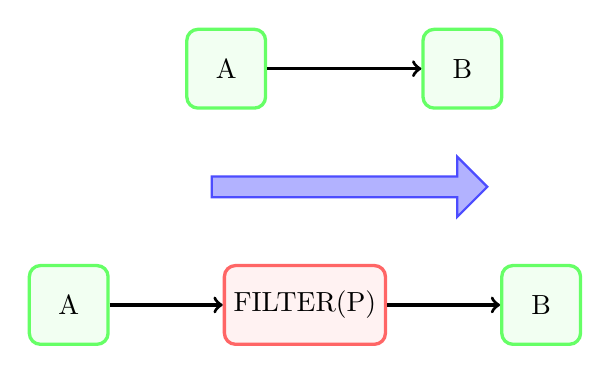
\begin{tikzpicture}[
redsquarednode/.style={rectangle, draw=red!60, fill=red!5, very thick, rounded corners, minimum size=10mm},
greensquarednode/.style={rectangle, draw=green!60, fill=green!5, very thick, rounded corners, minimum size=10mm},
fat arrow/.style={single arrow,thick,draw=blue!70,fill=blue!30,minimum height=35mm,minimum width=7mm}
]
%Nodes
\node[draw,greensquarednode] at (2,0) (SRC)    {A};
\node[draw,greensquarednode] at (5,0) (TARGET) {B};

\node at (3.5,-1.5) [fat arrow]{};

\node[draw,greensquarednode] at (0,-3) (SRC-1)    {A};
\node[draw,greensquarednode] at (6,-3) (TARGET-1) {B};
\node[draw,redsquarednode] at (3,-3) (FILTER) {FILTER(P)};

%Lines
\draw[->,very thick] (SRC.east) -- (TARGET.west);

\draw[->,very thick] (SRC-1.east) -- (FILTER.west);
\draw[->,very thick] (FILTER.east) -- (TARGET-1.west);
\end{tikzpicture}
\end{center}

%% \hspace*{10mm}\includegraphics[width=90mm,height=50mm]{filter.jpg}

If the data is valid, then it is passed on. Otherwise it is dropped.

\end{frame}


\begin{frame}\frametitle{Transformation: Message Monitoring}

A \emph{monitor} checks to see that a relationship $\mathcal{R}$ holds
over a collection of message streams through time. If the
specification is violated, an \emph{alert} is sent out.

\begin{center}
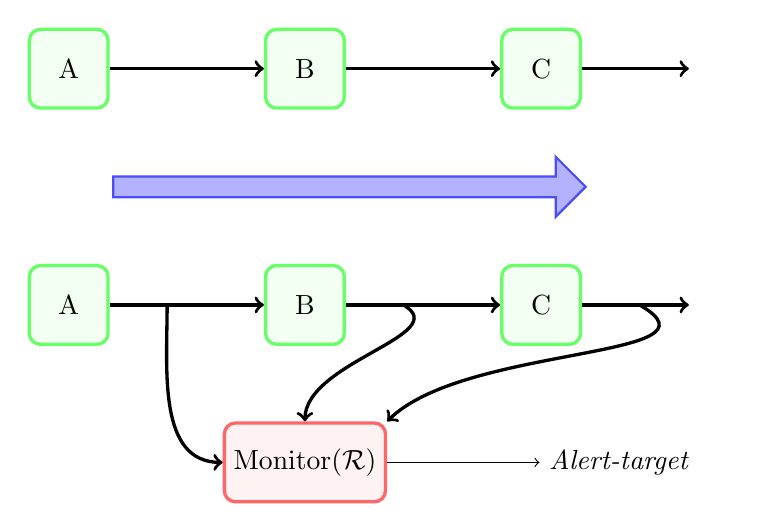
\begin{tikzpicture}[
redsquarednode/.style={rectangle, draw=red!60, fill=red!5, very thick, rounded corners, minimum size=10mm},
greensquarednode/.style={rectangle, draw=green!60, fill=green!5, very thick, rounded corners, minimum size=10mm},
fat arrow/.style={single arrow,thick,draw=blue!70,fill=blue!30,minimum height=60mm,minimum width=7mm}
]
%Nodes
\node[draw,greensquarednode] at (1,0) (A) {A};
\node[draw,greensquarednode] at (4,0) (B) {B};
\node[draw,greensquarednode] at (7,0) (C) {C};
\node at (9,0) (D) {};

\node at (4.5,-1.5) [fat arrow]{};

\node[draw,greensquarednode] at (1,-3) (A-1) {A};
\node at (2.25,-3) (joinAB) {};
\node[draw,greensquarednode] at (4,-3) (B-1) {B};
\node at (5.25,-3) (joinBC) {};
\node[draw,greensquarednode] at (7,-3) (C-1) {C};
\node at (8.25,-3) (joinCD) {};
\node at (9,-3) (D-1) {};
\node[draw,redsquarednode]   at (4,-5) (M) {Monitor($\mathcal{R}$)};
\node at (8,-5) (ALERT-TARGET) {\textit{Alert-target}};

%Lines
\draw[->,very thick] (A.east) -- (B.west);
\draw[->,very thick] (B.east) -- (C.west);
\draw[->,very thick] (C.east) -- (D.west);
\draw[->,very thick] (A-1.east) -- (B-1.west);
\draw[->,very thick] (B-1.east) -- (C-1.west);
\draw[->,very thick] (C-1.east) -- (D-1.west);

\draw[->,very thick] (2.25,-3) to [out=-90, in=180] (M);
\draw[->,very thick] (5.25,-3) to [out=-30, in=90]  (M);
\draw[->,very thick] (8.25,-3) to [out=-30, in=45]  (M.north east);
\draw[->] (M.east) -- (ALERT-TARGET);

\end{tikzpicture}
\end{center}

%% \hspace*{10mm}\includegraphics[width=90mm,height=40mm]{monitor.jpg}

\end{frame}

\begin{frame}\frametitle{Transformation: Message Monitoring}

 We currently use past-time temporal logic, encoded in Lustre, to
 specify monitor behavior. From that we synthesize implementations in CakeML.

\end{frame}


\begin{frame}\frametitle{Transformation: Isolation of `at risk' components}

An unprotected computational element can be isolated by transparently
lifting it out of its context and mediating access via seL4.

\begin{center}
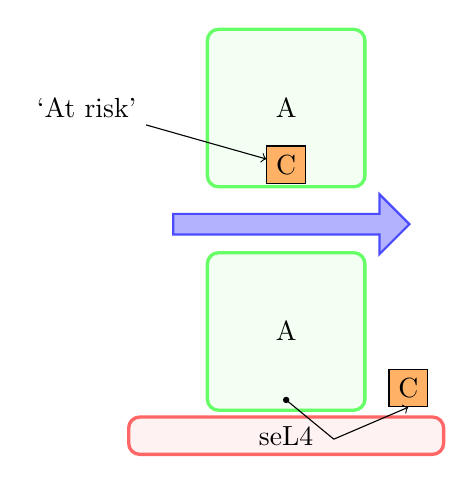
\begin{tikzpicture}[
bignode/.style =
  {rectangle,
   draw=green!60, fill=green!5,
   very thick, rounded corners,
   minimum height=20mm, minimum width = 20mm},
flatnode/.style =
  {rectangle,
   draw=red!60, fill=red!5,
   very thick, rounded corners,
   minimum width = 40mm},
fat arrow/.style={single arrow,thick,draw=blue!70,fill=blue!30,minimum height=30mm,minimum width=7mm}
]
%Nodes
\node[draw,bignode](main){A};
\node[draw,fill=orange!60] (atrisk) at ([yshift=2ex]main.south){C};
\node (comment) at ([xshift=-10ex]main.west){`At risk'};
\draw[->] (comment) -- (atrisk);
\node at ([yshift=-3ex]main.south) [fat arrow]{};
\node[draw,bignode](main-1) at ([yshift=-12ex]main.south){A};
\node[draw,fill=orange!60] (secure) at ([xshift=3.5ex,yshift=2ex]main-1.south east){C};
\node[draw,flatnode] (seL4) at ([yshift=-2ex]main-1.south){seL4};
\node[draw,fill=black,circle,scale = 0.2] (origin) at ([yshift=1ex]main-1.south){};
\node (foo) at ([yshift=-2ex,xshift=4ex]seL4.north){};
\draw (origin) -- (foo.center);
\draw[->] (foo.center) -- (secure.south);
\end{tikzpicture}
\end{center}

%\filldraw[black] (0,0) circle (2pt) node[anchor=west] {Intersection point};
%\hspace*{10mm}\includegraphics[width=90mm,height=40mm]{vm.jpg}

\end{frame}

\begin{frame}\frametitle{seL4}

Correctness of this transformation depends on formal guarantees provided by seL4.

\begin{itemize}
\item seL4 microkernel guarantees partitioning of components and
  communication, backed by computer-checked proofs

\item seL4 guarantees no infiltration, exfiltration, eavesdropping,
  interference, and provides fault containment for untrusted code

\end{itemize}

\vspace*{5mm}
\hspace*{10mm}\includegraphics[width=15mm,height=15mm]{data61-logo.png}
\hspace*{10mm}\includegraphics[width=15mm,height=15mm]{csiro--black.png}

\end{frame}

\begin{frame}\frametitle{Transformation: Attestation}

Attestation inserts measurement mechanisms into a system. These
examine various aspects of system behavior, and send summaries back to
an observer system.

%% %% \newcommand\rightEye[1][1.2ex]
%% %% {%
%% %% \begin{tikzpicture}[scale=#1/1cm]
%% %%   \draw (0,0) circle (.5);
%% %%   \fill (.25,0) circle (.25);
%% %% \end{tikzpicture}%
%% %% }

%% \begin{center}
%% \begin{tikzpicture}[
%% lefteyes/.style =
%%   {circle,
%%    draw=red!60, fill=red!5,
%%    minimum height=20mm, minimum width = 20mm}
%% ]
%% %Nodes
%% \draw (0,0) rectangle (1,1);
%% \draw (3,0) rectangle (1,1);

%% \draw (0,-3) rectangle (1,1);
%% \draw (3,-3) rectangle (1,1);
%% \draw (3,-3.5) rectangle (0.5,0.5);

%% \draw (3,-4) circle (.5);
%% \fill (3.25,-4) circle (.25);
%% \end{tikzpicture}
%% \end{center}

\hspace*{10mm}\includegraphics[width=90mm,height=40mm]{att.jpg}


\end{frame}

\begin{frame}\frametitle{CakeML implementations}

  The filter, monitor, and attestation transforms generate \konst{CakeML} implementations.

\begin{itemize}
 \item [$\blacktriangleright$] CakeML is a formally verified ML compiler

\item This allows a theorem that connects the high-level spec of a
  component with the execution of the binary on an ISA.
\end{itemize}

\end{frame}


\section{Technical Discussion}

\begin{frame}\frametitle{Contiguity Types}

  \emph{Contiguity types} provide a small but expressive DSL for
specifying message formats, especially those with
\kemph{self-describing} aspects such as length fields and
`unions'.

\vspace*{5mm}
Filters and parsers can be automatically generated from
contiguity type specifications, backed up by a formal correctness
proof.

\end{frame}

\begin{frame}\frametitle{Contiguity Types: Syntax and Semantics}

\[
\begin{array}{rcl}
 \tau & = & \konst{bool} \mid \konst{char} \mid \konst{u8} \mid
 \konst{u16} \mid \konst{u32} \mid \konst{u64}  \mid \konst{i16} \mid
 \konst{i32} \mid \konst{i64} \mid \ldots \\
      & \mid & \konst{Recd}\; (f_1 : \tau_1) \ldots (f_n : \tau_n) \\
      & \mid & \konst{Array}\; \tau \; \mathit{exp} \\
      & \mid & \konst{Union}\; (\mathit{bexp}_1 : \tau_1) \ldots (\mathit{bexp}_n : \tau_n)
\end{array}
\]


\[
% \begin{array}{l}
\LangTheta{\tau} =
\mathtt{case}\; \tau\
% \hspace*{3mm}
 \left\{
 \begin{array}{l}
 \mathit{base} \Rightarrow \set{s \mid \konst{len}(s) = \konst{width}(base)} \\
 \konst{Recd}\; (f_1 : \tau_1) \ldots (f_n : \tau_n)
      \Rightarrow \LangTheta{\tau_1} \cdot \ldots \cdot \LangTheta{\tau_n}
\\
 \konst{Array}\; \tau_1 \; \mathit{exp}
      \Rightarrow  \LangTheta{\tau_1}^{\konst{evalExp}\;\theta\;\mathit{exp}}
\\
 \konst{Union}\; (\mathit{bexp}_1 : \tau_1) \ldots (\mathit{bexp}_n : \tau_n) \Rightarrow \\
  \hspace*{5mm}
 \left\{
 \begin{array}{ll}
    \LangTheta{\tau_i} &  \mathrm{if}\ \konst{evalBexp}\;\theta\;\mathit{bexp}_i = \konst{true} \\
                  & \mathrm{and\ no\ other}\ \mathit{bexp}_j\ \mathrm{is}\ \konst{true}  \\
    \emptyset & \mathrm{otherwise}
 \end{array}
 \right.
 \\
\end{array}
 \right.
%\end{array}
\]

\end{frame}

\begin{frame}\frametitle{Application in CASE}

In CASE, contiguity types have been used to implement the
\kemph{insert-filter} and \kemph{insert-monitor} architectural
transformations for the set of UxAS message types.

\vspace*{5mm}

UxAS messages can be very large and complex; contiguity types handled
them straightforwardly, with only some minor workarounds.

\vspace*{5mm}
(Our current work will eliminate the workarounds)

\end{frame}

\begin{frame}[fragile]\frametitle{Example: $A^n B^n C^n$}

{\small
\begin{verbatim}
  charA = {ch : char, isA : Assert (ch = 97)}
  charB = {ch : char, isB : Assert (ch = 98)}
  charC = {ch : char, isC : Assert (ch = 99)}

  mesg = {len : u16
            A : charA [len]
            B : charB [len]
            C : charC [len]
          }
\end{verbatim}
}

\[
\Lang{\mathit{mesg}} = u \cdot A^{\konst{val}(u)} \cdot B^{\konst{val}(u)} \cdot C^{\konst{val}(u)} \]

\end{frame}


\begin{frame}[fragile]\frametitle{Example: 2D array of GPS coords}

{\small
\begin{verbatim}
 AltitudeType = AGL | MSL

 Location3D = {
  Latitude  : double,
  Longitude : double,
  Altitude  : float,
  AltitudeType : AltitudeType,
  Wellformed : Assert (
      -90.0 <= Latitude <= 90.0 and
     -180.0 <= Longitude <= 180.0 and
      0.0 <= Altitude <= 15000.0)
  }

 Locations = {
    dims : {rows u16, cols : u16}
   table : Location3D [dims.rows * doms.cols]
  }
\end{verbatim}
}
\end{frame}


\begin{frame}\frametitle{Key innovations in contiguity types}

\begin{itemize}

\item [$\blacktriangleright$] \kemph{Systematic accumulation and
  exploitation of context.} As a contiguity type parser processes a
  message, each field is added to the context. Context is
  used in the computation of length fields, and in calculating which
  element of a union to choose.

\item [$\blacktriangleright$] \kemph{Context-sensitive sum.} There is
  no unadorned `sum' operation $L_1 \cup L_2$. Instead, we have a
  `guarded union` type
  $\konst{Union}\; (\mathit{bexp}_1 : \tau_1) \ldots (\mathit{bexp}_n : \tau_n)$
  where evaluation of the $\mathit{bexp}_i$, in the accumulated
  context, is used to determine which $\tau_i$ to continue parsing
  with.

\item [$\blacktriangleright$] \kemph{In-message assertions} Message
  constraints can be expressed within a contiguity type. This allows
  data constraints to be expressed alongside the data in the message
  specification.

\end{itemize}
\end{frame}

\begin{frame}\frametitle{Key innovations in contiguity types (contd)}

\begin{itemize}

\item [$\blacktriangleright$] \kemph{Message fields = memory
  locations.}  A contiguity type specification for a message format
  superimposes a C-like memory view on a message. Array length
  expressions and boolean choices in sums use R-values to compute
  values over already-seen message fields. This gives `dependent type'
  specification power without dependent types.

\item [$\blacktriangleright$] \kemph{Work at the string/byte buffer
  level.}  This allows us to avoid lifting message components to real
  types unnecessarily, \eg, when doing pure recognition as in a
  filter.

\end{itemize}
\end{frame}


\begin{frame}\frametitle{Generalized Contiguity Types}

We are in the process of replacing the base types with a lexer and
adding unbounded lists (a form of Kleene Star):

\[
\begin{array}{rcl}
 \tau & =    & \highlight{\konst{Base}\; (\mathit{regexp} \times \mathit{valFn})} \\
      & \mid & \konst{Recd}\; (f_1 : \tau_1) \ldots (f_n : \tau_n) \\
      & \mid & \highlight{\konst{List}\; \tau} \\
      & \mid & \konst{Array}\; \tau \; \mathit{exp} \\
      & \mid & \konst{Union}\; (\mathit{bexp}_1 : \tau_1) \ldots (\mathit{bexp}_n : \tau_n)
\end{array}
\]

The lexer will support all the original fixed-width base types, along
with common lexemes for unbounded numbers, string literals, and
\adhoc{} field widths for packed encodings.

\end{frame}


\begin{frame}[fragile]\frametitle{List types}

The \kemph{List} constructor is used for parsing structures where the
number of elements is unknown at the outset.

\begin{itemize}

\item [$\blacktriangleright$] Encoded as a sequence of \konst{ConsTag}ed elements
  terminated with a \konst{NilTag}:

\[
  \konst{List}\, \tau = \konst{ConsTag} \cdot \tau \cdots \konst{ConsTag} \cdot \tau \cdot \konst{NilTag}
\]

\item [$\blacktriangleright$] More complex structures are built on
  lists. For example, arithmetic expressions, logic formulas, program
  syntax trees.

\item [$\blacktriangleright$] Compositional: construction of
  (generalized) contiguity types is closed under $\konst{List}$, so
  has a strong connection with Kleene star, which is used as a closure
  operator for formal languages.

\end{itemize}
\end{frame}


\begin{frame}[fragile]\frametitle{Example: first order terms}

Can be described by the following datatype:

{\small
\begin{verbatim}
  term = Var of string
       | App of string * term list
\end{verbatim}}

A contiguity type for this would be

{\small
\begin{verbatim}
  term = {
    tag : u8
    kind : Union {
           tag = VarTag ==> {varName : string}
           tag = AppTag ==> {fnName : string, Args : List term}}
   }
\end{verbatim}}

It would be useful to create a `compiler' from the above kinds of
(recursive) datatype definitions to the corresponding contiguity type.

\end{frame}

\begin{frame}\frametitle{Combination with conventional parser technology}

  What we have is a type-directed and context-oriented parser
  generator that has some similarities with LL(0) or LR(0) languages
  wherein the parser can proceed with no lookahead.

\begin{itemize}

\item  [$\blacktriangleright$] This is useful for binary-encoded datastructures.

\item [$\blacktriangleright$] Can it be generalized to use lookahead
  to handle more complex, text-based representations of data such as
  JSON?

\item [$\blacktriangleright$]
\kemph{Idea (Hardin)} Can we `lift' so that contiguity types are
  used to specify the lexeme level, and use (say) an LR parser
  generator to handle higher-level grammar elements?
\end{itemize}

\end{frame}


\begin{frame} \frametitle{Verification Story}

\begin{itemize}

\item [$\blacktriangleright$] Proved parser generator sound (every
  successfully parsed message is in the language of the given
  contiguity type).

\item [$\blacktriangleright$] We are integrating a pre-existing
  max. munch lexer generator. (Formal correctness proof from previous
  work with Scott Owens).

\item [$\blacktriangleright$] We have existing SLR and PEG parsers
  that are formally verified, and want to integrate with them.

\end{itemize}

\end{frame}

\section{Applications and Future Directions}

\begin{frame} \frametitle{Compilation}

\begin{itemize}

\item [$\blacktriangleright$] The contig. type parser generator
  operates in an essentially \kemph{interpreted} mode.

\item [$\blacktriangleright$] Our generated filters in CASE can keep
  up with the rest of the system, but we would like to have filters
  and monitors that run at max. speed.

\item [$\blacktriangleright$] We know how to \kemph{compile}
  contig. types and would like to implement this translator, prove
  it correct, and apply to challenging examples.

\end{itemize}

\end{frame}


\begin{frame} \frametitle{Modular parsing}

SafeDocs has shown that difficult languages such as PDF can involve
multiple sub-languages, which may need coordination in their
parsing.

\begin{itemize}

\item [$\blacktriangleright$] What seems to be needed is a way to---in
  the midst of parsing language $A$---select a subsequence of the
  input to separately parse with the parser for language $B$.

\item [$\blacktriangleright$] In
  determining the slice of the input to give to $B$, the accumulated
  context often needs to be consulted.

\item [$\blacktriangleright$] Contiguity types give a way to handle
  this, and, in particular, may also offer a framework in which the
  context accumulated by $B$ is added back to that of $A$.

\end{itemize}

\end{frame}


\begin{frame}\frametitle{Interesting Directions}

\begin{itemize}

\item [$\blacktriangleright$] System modelling as `boxes and arrows'
  where the arrows are specified by contiguity types. Thus would get
  an interesting overview of the message formats in the system, early
  on in design. Are there interesting security analyses that can be
  done at that point? Probably we will need to add some behavior to
  the boxes. (Currently doing just this in CASE.)


\item [$\blacktriangleright$] Auto-generation of test suites and harnesses from contig. type specs.

\item [$\blacktriangleright$] New and challenging examples

\item [$\blacktriangleright$] Others?

\end{itemize}

\end{frame}


\end{document}
